\documentclass[11pt]{article}
\oddsidemargin -0.0in
\topmargin -0.5in
\textwidth 6.25in
\textheight 9.25in
\setlength\parindent{0pt}
\usepackage{graphicx} % need this package

\begin{document}

\title{CSCI347, Winter 2019, Matrix Multiplication with Threads\\Rose Lim}
\maketitle

To implement the pthreads, I split up the amount of results needed to calculate (x * z) by the number of threads (t) and named it "part". 
The last thread could have part+1.
\\ 
\\
For matrix multiply, each thread knew its start position (which would be the thread id multiplied by by the "part" variable from before) and end position (start position + "part"). 
These numbers could be converted into column and row by dividing it by x and also using its remainder. 
Do the calculation from start position to end position, then the thread would return. 
\\
\\
For matrix square, the concept is the same with the start and end position, however, the first thread would keep count of how many squares the matrix has done. 
After each thread is done computing, it does a barrier wait until all threads are finished, then it calls itself to square again as many times as needed.
\\
\\
For experiements, I used the lab machines to run both the original code and my threaded code at different sizes of matricies. I graphed with excel. 
\\
\\
\begin{figure}[htbp]
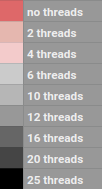
\includegraphics[scale = .4]{C:/Users/miles/Downloads/cs/347/csci347_w19/mm/key.png}
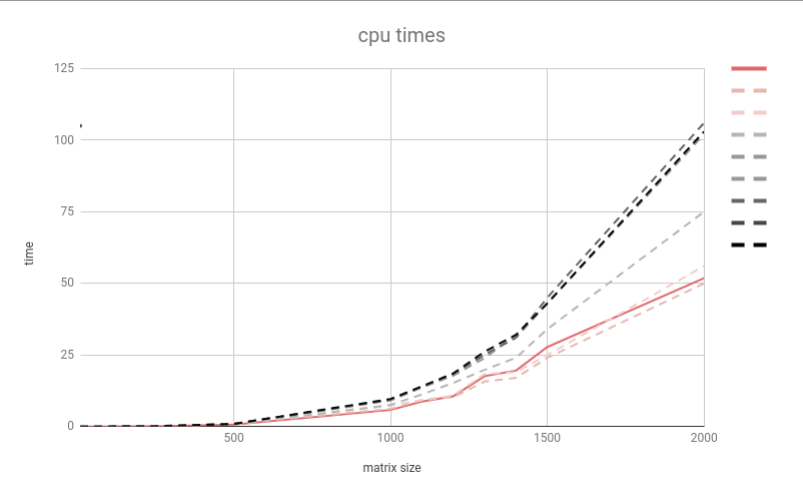
\includegraphics[scale = .4]{C:/Users/miles/Downloads/cs/347/csci347_w19/mm/cpu_time.png}
\caption{with CPU time, the higher amount of thread takes up more time.}
\end{figure}
\\
\begin{figure}[htbp]
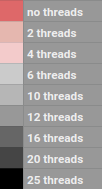
\includegraphics[scale = .4]{C:/Users/miles/Downloads/cs/347/csci347_w19/mm/key.png}
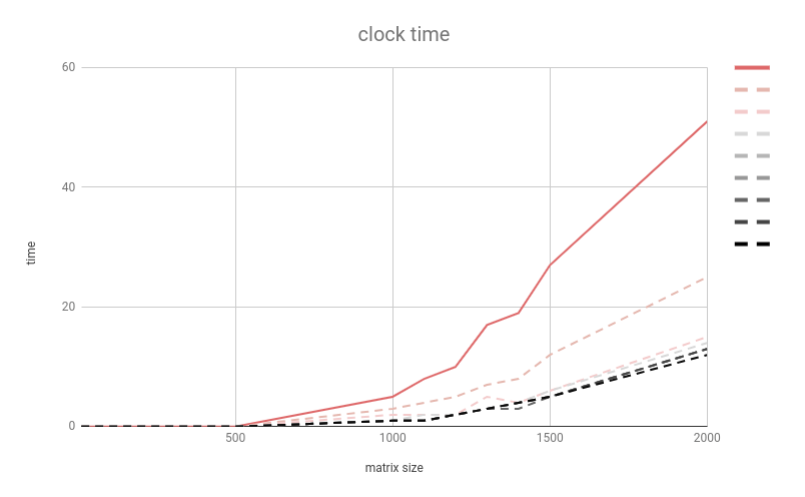
\includegraphics[scale = .4]{C:/Users/miles/Downloads/cs/347/csci347_w19/mm/clock_time.png}
\caption{with real time, starting at a matrix over 500x500, more threads seems to correlate with less computation time.}
\end{figure}
\\
\begin{figure}[htbp]
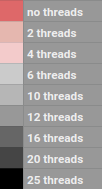
\includegraphics[scale = .4]{C:/Users/miles/Downloads/cs/347/csci347_w19/mm/key.png}
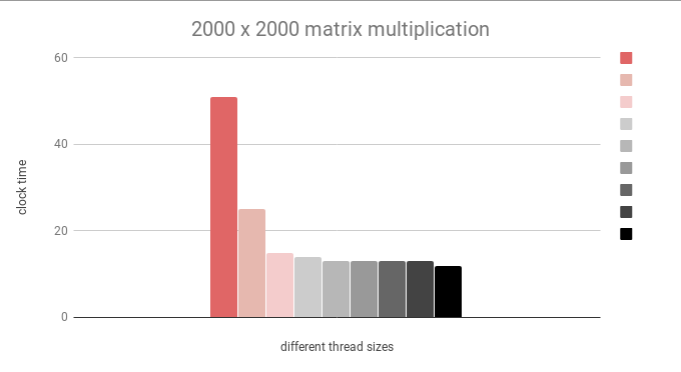
\includegraphics[scale = .4]{C:/Users/miles/Downloads/cs/347/csci347_w19/mm/2000x2000.png}
\caption{From 0 threads to 2 threads, the amount of time it takes to calculate almost decreases by half. From 2 threads to 4 threads, the amount of time it takes to calculate is close to half. Adding more threads from there does not show a dramatic speedup in time, just about a few seconds less.}
\end{figure}

I did not expect the CPU time to be increasing, but it makes sense because it is creating all the threads. I expected my threaded code to be faster than no threads, but I did not expect the exponential decrease in efficiency as more threads were added. \\
\\
All in all, threads are pretty neat and when a matrix more than 500x500 is being multiplied with another matrix more than 500x500, multiple threads splitting up the work could be very efficient. More threads could be more efficient, however, at around 6 or 8 threads, the efficiency is less relevant, which explains why my program defaults to 8 threads. 

\end{document}